\section{Spatial-Spark}

% \subsection{空间数据分析处理}

% \begin{frame}[t]{Spatial-Spark}
%     \begin{columns}
%         %Transform and projection
%         \begin{column}{0.4 \textwidth}

%             \begin{center}
%             \alert{Proj.4}

%             \begin{itemize}
%                 \item 空间椭球基础
%                 \item 空间参照系统
%                 \item 空间投影系统
%                 \item 坐标换算
%             \end{itemize}
%             \end{center}
            
%         \end{column}
%         % JTS
%         \pause
%         \begin{column}{0.6 \textwidth}

%             \begin{center}
%              \alert{JTS Topogy Suite}

%                 \begin{itemize}
%                 \item 简单空间要素类型
%                 \item 空间数据分析和空间运算
%                 \item 空间数据读写
%                 \end{itemize}
%             \end{center}
           
%         \end{column}
%     \end{columns}
% \end{frame}

\subsection{Spatial-Spark}


\begin{frame}[c]{体系结构}
    \begin{center}
        \alert{Spatial-Spark体系结构}
    

    \vspace{1em}
    \begin{figure}
        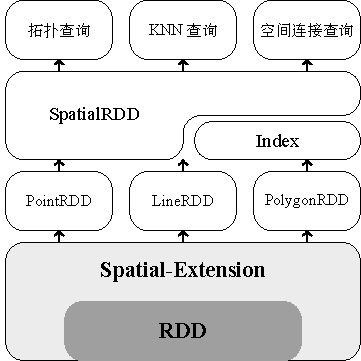
\includegraphics[scale=1.0]{figures/spatialspark.pdf}
    \end{figure}
    \end{center}
\end{frame}


\begin{frame}[t]{辅助模块}
    \begin{columns}
        %Transform and projection
        \begin{column}{0.4 \textwidth}

            \begin{center}
            \alert{Proj.4}

            \begin{itemize}
                \item 空间椭球基础
                \item 空间参照系统
                \item 空间投影系统
                \item 坐标换算
            \end{itemize}
            \end{center}
            
        \end{column}
        % JTS
        \pause
        \begin{column}{0.6 \textwidth}

            \begin{center}
             \alert{JTS Topogy Suite}

                \begin{itemize}
                \item 简单空间要素类型
                \item 空间数据分析和空间运算
                \item 空间数据读写
                \end{itemize}
            \end{center}
           
        \end{column}
    \end{columns}
\end{frame}

\begin{frame}[c]{RDD空间扩展}
    PointRDD、LineRDD和PolygonRDD

    Spatial-RDD
    \pause
    \begin{itemize}
        \item HDFS中读取
    \end{itemize}
    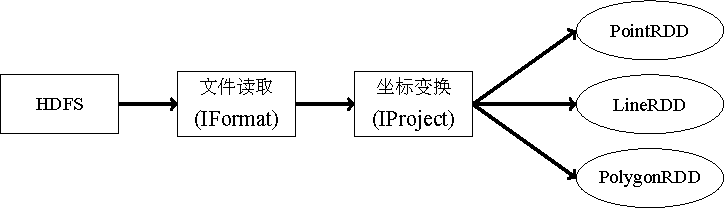
\includegraphics[scale=0.8]{figures/spatialRDD.pdf}

    \pause
    \begin{itemize}
        \item Spatial-RDD空间运算相互转换
    \end{itemize}
\end{frame}

\begin{frame}[c]{空间索引}
    \begin{columns}
        \begin{column}{0.6 \textwidth}
        R树空间索引

        \vspace{1em}
        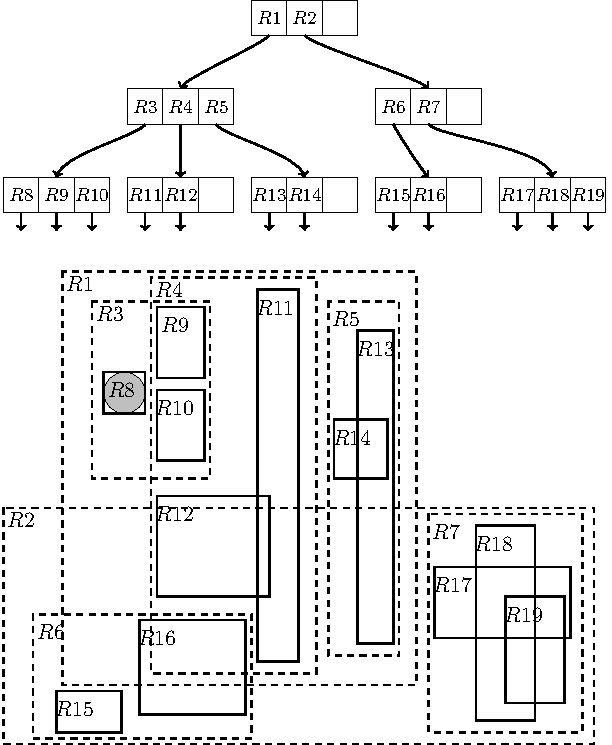
\includegraphics[scale=0.4]{figures/rtree.pdf}
        \end{column}

        \pause
        \begin{column}{0.4 \textwidth}
            \begin{itemize}
                \item R树插入
                \pause
                \item R树查询
                    \begin{itemize}
                        \pause
                        \item 过滤
                        \pause
                        \item 精选
                    \end{itemize}
            \end{itemize}
        \end{column}
    \end{columns}
\end{frame}

\begin{frame}[c]{空间查询}
    \begin{itemize}
        \item \alert{空间拓扑查询}
    \end{itemize}
    支持Spatial-RDD之间的所有拓扑操作

    \pause
    \begin{itemize}
        \item \alert{空间KNN查询}
    \end{itemize}
    借助优先级队列,筛选K个邻居;可借助索引加速空间查询

    \pause
    \begin{itemize}
        \item \alert{空间连接查询}
    \end{itemize}
    过滤步骤;精选步骤
\end{frame}
\subsection{实验分析}

\begin{frame}[t]{实验分析}
    MapReduce与Spatial-Spark空间过滤筛选对比
    \vspace{1em}
    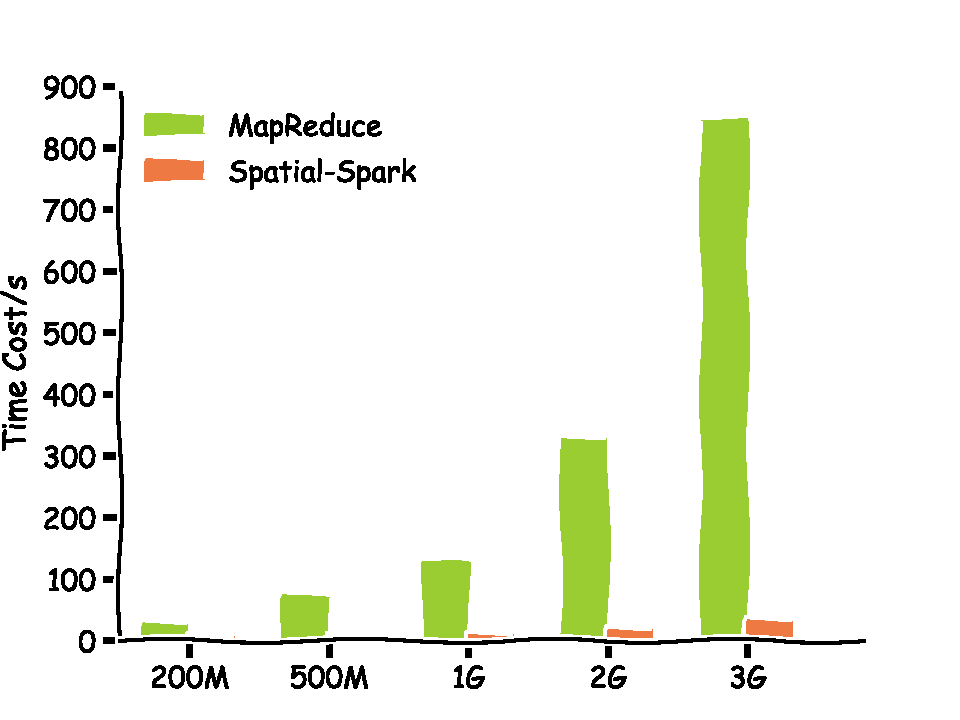
\includegraphics[width=0.9 \textwidth]{figures/topo_query.pdf}
\end{frame}

\begin{frame}[t]{实验分析}
    Spatial-Spark集群扩展性能分析
    \vspace{1em}
    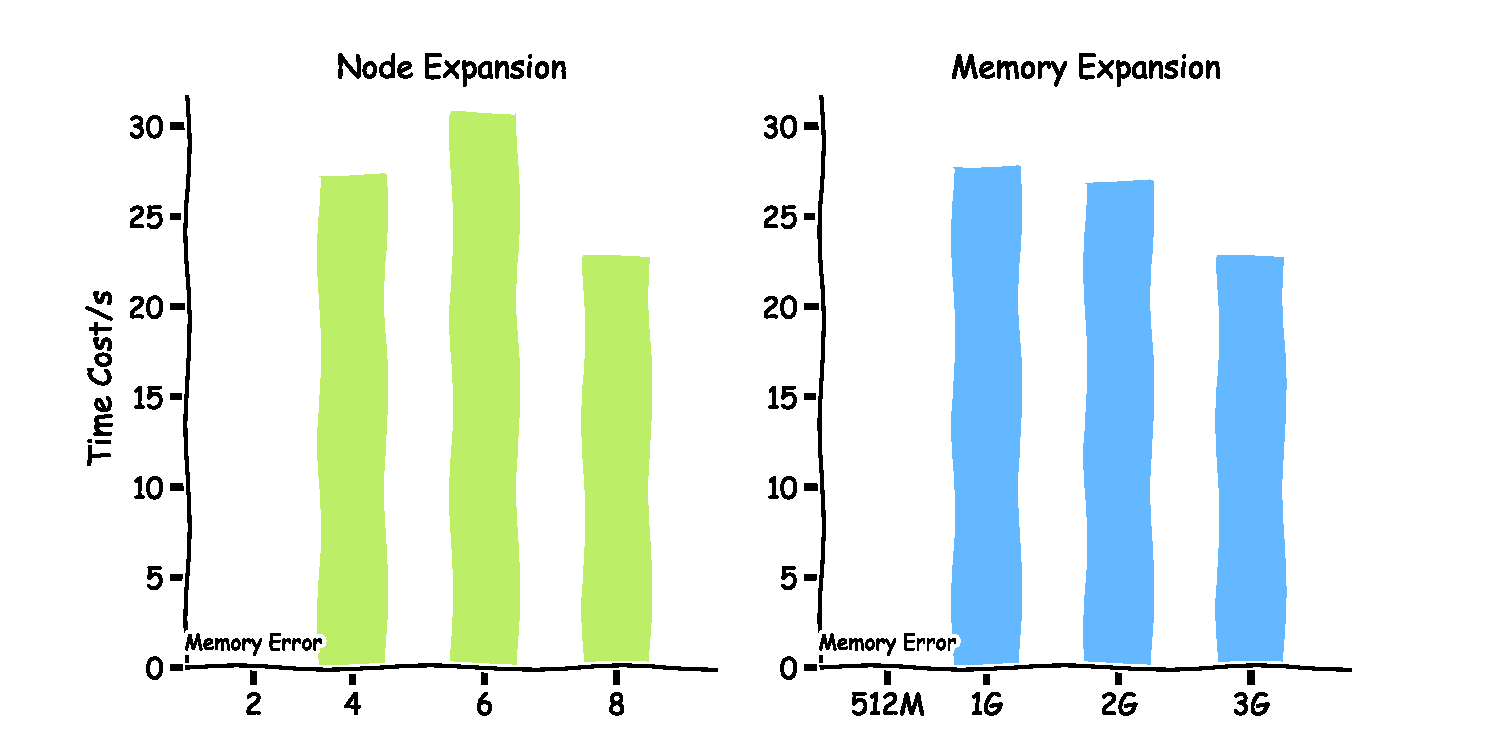
\includegraphics[width=0.9 \textwidth]{figures/node_memory.pdf}
\end{frame}

\begin{frame}[t]{实验分析}
    Spatial-Spark 空间索引性能分析
    \vspace{1em}
    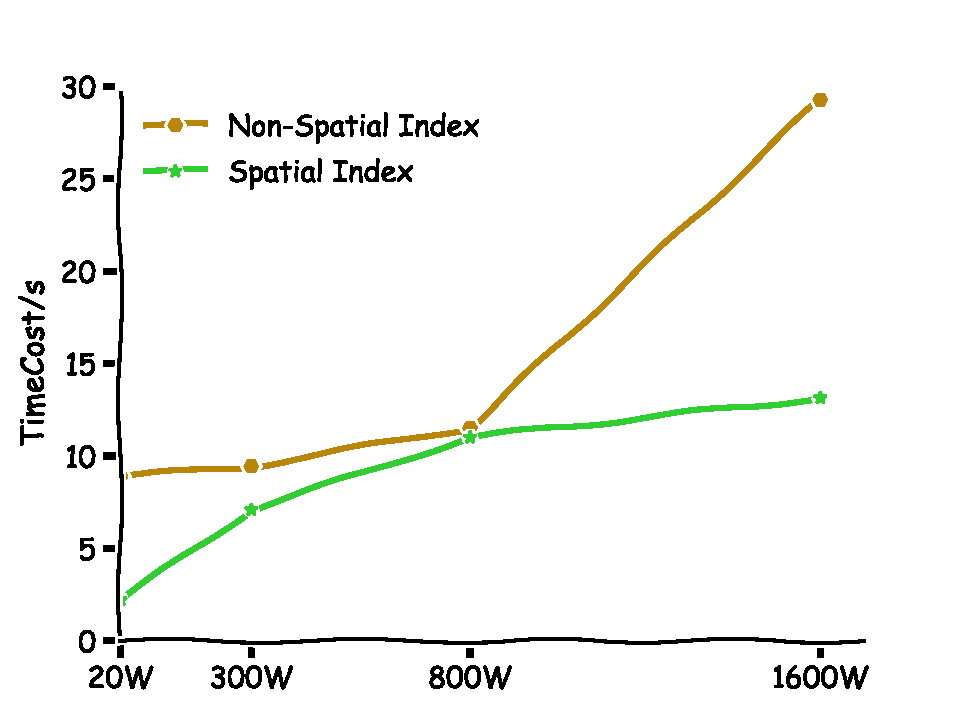
\includegraphics[width=0.9 \textwidth]{figures/index.pdf}
\end{frame}


